% !TEX TS-program = pdflatex
% !TEX encoding = UTF-8 Unicode

% This is a simple template for a LaTeX document using the "article" class.
% See "book", "report", "letter" for other types of document.

\documentclass[11pt]{article} % use larger type; default would be 10pt

\usepackage[utf8]{inputenc} % set input encoding (not needed with XeLaTeX)

%%% PAGE DIMENSIONS
\usepackage{geometry} % to change the page dimensions
\geometry{a4paper} % or letterpaper (US) or a5paper or....
% \geometry{margin=2in} % for example, change the margins to 2 inches all round
% \geometry{landscape} % set up the page for landscape
%   read geometry.pdf for detailed page layout information

\usepackage{graphicx} % support the \includegraphics command and options

% \usepackage[parfill]{parskip} % Activate to begin paragraphs with an empty line rather than an indent

%%% PACKAGES
\usepackage{booktabs} % for much better looking tables
\usepackage{array} % for better arrays (eg matrices) in maths
\usepackage{paralist} % very flexible & customisable lists (eg. enumerate/itemize, etc.)
\usepackage{verbatim} % adds environment for commenting out blocks of text & for better verbatim
\usepackage{subfig} % make it possible to include more than one captioned figure/table in a single float
% These packages are all incorporated in the memoir class to one degree or another...

%%% HEADERS & FOOTERS
% \usepackage{fancyhdr} % This should be set AFTER setting up the page geometry
% \pagestyle{fancy} % options: empty , plain , fancy
% \renewcommand{\headrulewidth}{0pt} % customise the layout...
% \lhead{}\chead{}\rhead{}
% \lfoot{}\cfoot{\thepage}\rfoot{}

%%% SECTION TITLE APPEARANCE
\usepackage{sectsty}
\allsectionsfont{\sffamily\mdseries\upshape} % (See the fntguide.pdf for font help)
% (This matches ConTeXt defaults)

%%% ToC (table of contents) APPEARANCE
\usepackage[nottoc,notlof,notlot]{tocbibind} % Put the bibliography in the ToC
\usepackage[titles,subfigure]{tocloft} % Alter the style of the Table of Contents
\renewcommand{\cftsecfont}{\rmfamily\mdseries\upshape}
\renewcommand{\cftsecpagefont}{\rmfamily\mdseries\upshape} % No bold!

% Package to insert code
\usepackage{xcolor}
\usepackage{listings}
\newcommand{\classname}[1]{\texttt{#1}}

%%% END Article customizations

%%% The "real" document content comes below...

\title{BGLgeom library}
\author{Speranza Ilaria (matr. 854196) \\ Tantardini Mattia (matr. 858603)}
%\date{} % Activate to display a given date or no date (if empty),
         % otherwise the current date is printed 

\begin{document}
\maketitle
\newpage
\tableofcontents
\newpage

\section{Introduction}
	\subsection{Purpouse of the project}	%magari anche no??
	The purpose of the project is to extend the Boost Graph Library (BGL) providing it more functionalities to handle graph with geometric properties, that the BGL currently does not support. This mainly means to provide a graph from BGL, that already implements all topological operations, a way to describe its vertices as points and its edges as curves in the space (2 or 3 dimensional). Along with this, classes which implements these kind of geometrical properties must be able to carry out geometric and analytic operations, such as computation of first and second derivative of the edges and creation of numerical meshes on them. \newline
	All these geometric functionalities we developed are aimed at solving numerical problems which can be modelled using a graph, but which also are in a geometric setting or need it: for instance, to compute flows in a network of blood vessels, meshes are required to solve finite element problemst. \newline
	Along with this library we provide to example of specific application: one about intersection of fractures in fractured porous media, and one solving a simple diffusion problem on a vascular network. \newline
	A lot of other applications can take advantage from this library: vascular and neural network, electronic circuits, .... 


\section{The library}
	\subsection{Briefs on BGL}
	The BGL is a template library to create, handle and operate on graphs. It implements some different classes of graphs, all the topological operations concerning graphs, and a lot of graph algorithms.
	\newline\newline
	% Metto qui quello che ho messo nella documentazione? adjacency_list e tutto il resto? forse comunque ho bisogno di dire dell'adjacency list, ma
	Among all these functionalities, we decide to concentrate on a single class to describe a graph and on how implement in an easy to use way the geometrical properties. To explain in more details our implementation choices, we need to spend some words on how that class and the graph properties work.
	
		\subsubsection{The adjacency\_list class}
		\classname{adjacency\_list} is a template class which represents a graph with a two dimensional structure: 
		a \texttt{VertexList} and a \texttt{OutEdgeList} container. The first one stores all the vertices of the graph, and each vertex contains the other one-dimensional structure which is the list of all the out-edges leaving that vertex (so only out-edges if the graph is directed, all the edges if the graph is undirected). \newline
		The class has five template parameters and the full protoytpe is: \classname{adjacency\_list< OutEdgeList, VertexList, Directed, VertexProperties, EdgeProperties >}. \newline
		The first two template parameters allow to choose the types of the underlying containers for the bidimensional structure. Choosing them affects space complexity of the graph and efficiency of some operations, such as inserting and removing edges. In our work we always set them to the selector \classname{boost::vecS} (that stands for \texttt{std::vector}) for ease of use and since, form BGL documentation, it is in average the most performant choice for every topological operation. \newline
		The third template parameter obviously allows to choose between a directed or undirected graph.\newline
		The last two template parameters are the most interesting ones. 
		
		
		\begin{itemize}
			\item \texttt{OutEdgeList}: here you can choose which container to use for this 
			structure. We recommend to use @a boost::vecS (that refers to the 
			std::vector). As alternative, if you have to perform a lot insertions 
			and removals of vertices and edges, you can choose @a boost::listS 
			(that refers to std:list), that is slightly more efficient for this 
			type of operations.
			
			\item \texttt{VertexList} 
		\end{itemize}
		 
	
	\subsection{BGLgeom}
	% Mettere delle subsubsection con tipo le classi principali, cosa fanno, perché fatte così, ecc
		\subsubsection{Vertex\_base\_property}
		
		\subsubsection{Edge\_base\_property}
	
	\subsection{Todos}	%???


\section{Applications}

	In this section we present two examples from real situations, where some tools of BGLgeom library prove to be useful.

	\subsection{Fracture Intersection}
		In this example a list of fractures, all lying on the same plane, is given as input. The goal is to build a graph representing the network, with vertices in correspondence of the fractures' extremities and of the intersection points  and edges representing the fractures. 
		\begin{figure}
			\centering 
			%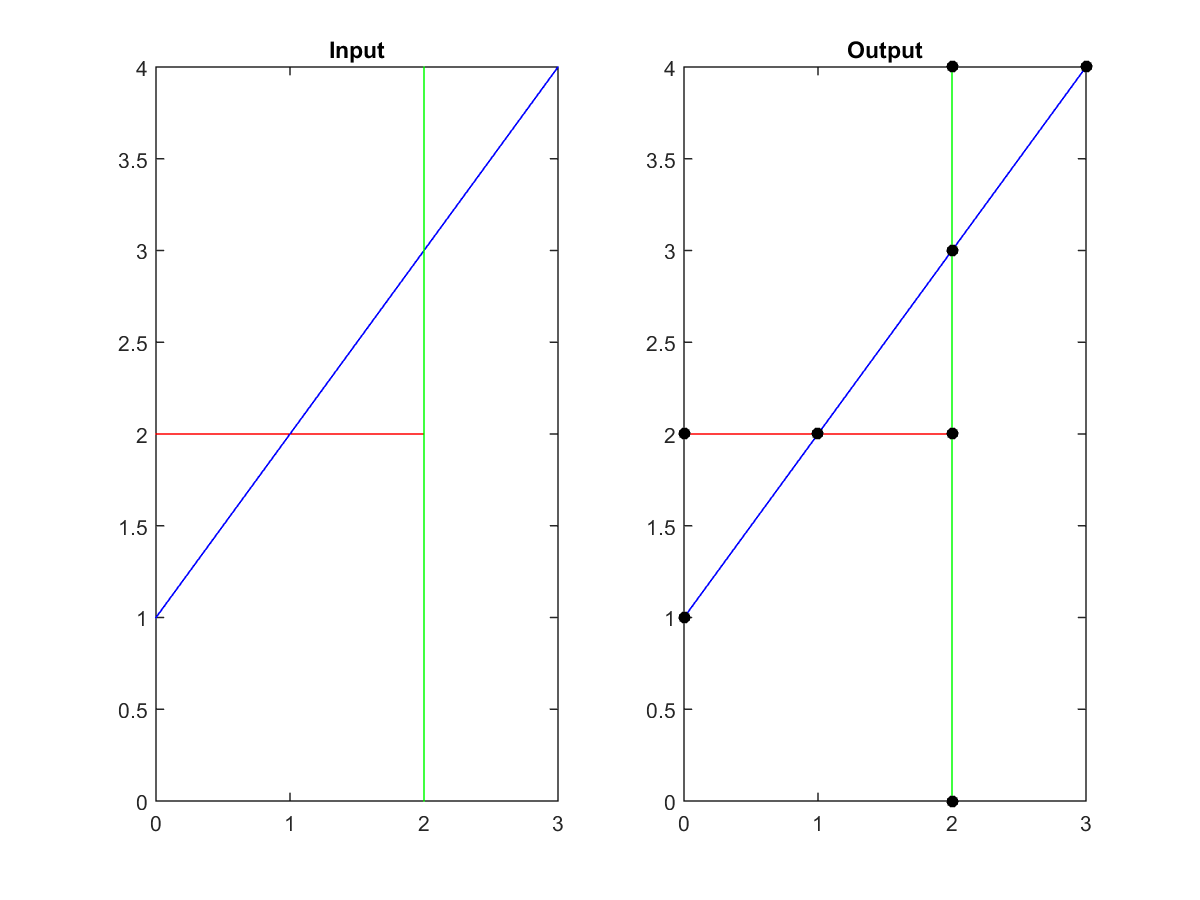
\includegraphics[width=0.5\textwidth]{frac_inters}
			\caption{Example}
			\label{fig:frac_int}
		\end{figure}



	\subsection{Diffusion on vascular network}


\end{document}
